\documentclass[11pt]{article}

\usepackage{amsmath}
\usepackage{graphicx}
\usepackage{multicol}
\usepackage{natbib}
\usepackage{wrapfig}
\usepackage{hyperref}
\usepackage{tabularx}
\usepackage{setspace}
\usepackage{comment}
\usepackage{color}

\usepackage[compact]{titlesec}  
\titlespacing{\section}{0pt}{0pt}{0pt}
\titlespacing{\subsection}{0pt}{0pt}{0pt}
\titlespacing{\subsubsection}{0pt}{0pt}{0pt}

\oddsidemargin 0cm
\evensidemargin 0cm

\usepackage[margin=1in]{geometry}

\parindent 0cm
\parskip 0.5cm

\usepackage{fancyhdr}
\pagestyle{fancy}
\fancyhf{}
%\fancyhead[L]{AOSS Reference Sheet}
\fancyhead[C]{\small Projecting future changes to lifecycle characteristics of North Atlantic cyclones}
\fancyfoot[C]{Page \thepage}

\newcommand{\vb}{\mathbf}
\newcommand{\diff}[2]{\frac{d #1}{d #2}}
\newcommand{\diffsq}[2]{\frac{d^2 #1}{{d #2}^2}}
\newcommand{\pdiff}[2]{\frac{\partial #1}{\partial #2}}
\newcommand{\pdiffsq}[2]{\frac{\partial^2 #1}{{\partial #2}^2}}
\newcommand{\topic}{\textbf}
\newcommand{\arcsinh}{\mathrm{arcsinh}}
\newcommand{\arccosh}{\mathrm{arccosh}}
\newcommand{\arctanh}{\mathrm{arctanh}}

\begin{document}

\appendix

\addtocounter{section}{3}


\begin{comment}
%\section*{Notes}
- African Easterly Waves
- Why does the number of cyclones decrease in the future?  Is this robust across models (but high resolution is needed)?  Humidity at 600hPa; shearing differences?  SST distribution?
- Focus on the northern Atlantic and eastern Pacific
- Why does intensity increase?
- Are coupled model simulations needed to assess tropical cyclones?  Coupled model biases are very problematic
- Extratropical cyclones and the tropical transition.  Is the tropical transition pushed farther North?  Detection algorithm based approach to ETCs.
- An outcome is a more robust detection / stitching algorithms
- Changes in landfall?  Assessment of regions which will be more susceptible to TC damage.  How does recurving affect this?
- "Changes in global circulation and the effect on local extremes"
- Leverage the ensemble of high resolution ensemble data
- Variable resolution over the Atlantic basin; run a bunch of ensembles at 25 km resolution
- What are the resolution dependencies of ETCs?
- Characterizing changing t-storms (size, wind speed, pressure, symmetry, latitude of max intensity, precipitation, latitude of maximum intensity, precipitation over land)
- Characterizing changing et-storms (size, wind speed, pressure, snow/rain precip. amounts, latitude of max. intensity)
\end{comment}
 
\section{Project Description}

The next century will see unprecedented changes to the climate system with direct socioeconomic repercussions.  These impacts will be particularly apparent from extreme weather events: As stated in the Third National Climate Assessment \citep{ThirdNCA}, ``changes in extreme weather events are the primary way that most people experience climate change.''  Changes to the character of extreme weather events have been observed since at least 1950, and have been at least partially linked to climate change due to human influences \citep{IPCCAR5WGI}.  In this sense, the characteristics of climate extremes are key indictors of climate change, and addressing observed and projected changes in these quantities will be crucial for future climate assessments.

In this work, we propose to address the complete lifecycle of one particular type of extreme weather event -- \textbf{North Atlantic basin tropical cyclones}.  Storms in this region are responsible for significant economic and social costs from flooding, property damage and fatality.  Hurricane Sandy, which impacted the New Jersey Coast in 2012, cost an estimated \$68 billion dollars and was responsible for 233 deaths \citep{Blake2012Report}.  Hurricane Katrina, which impacted New Orleans in 2005, cost an estimated \$108 billion dollars and was responsible for 1833 deaths \citep{Knabb2005Report}.  Our goal is to understand the characteristics of these storms under projections of future climate over their lifetime, including cyclogenesis, mid-life and termination (either via landfall or extratropical transition).  This proposal  further aims to explain the physical drivers behind reported reductions in North Atlantic tropical cyclone counts that have been observed in past studies.

The key scientific questions that are the focus of this proposal are as follows:
\begin{itemize}
\item[(Q1)] Is the location of tropical cyclogenesis in the North Atlantic basin modified under climate change in high-resolution climate model simulations? How does the projected intensification of the African Easterly Jet impact cyclogenesis off the African coast?

\item[(Q2)] How are the lifetime characteristics of tropical cyclones, including wind intensity, size, precipitation, and spatial density of storms affected under future climate change in high-resolution climate model simulations?

\item[(Q3)] Is there a change in the character, including location and frequency, of tropical cyclones undergoing an extratropical transition?

\item[(Q4)] How are cyclone trajectories, probability of landfall, location of landfall and total overland precipitation affected under future climate change? 
\end{itemize}

The central hypotheses of this proposal are as follows:

\vspace{-0.4cm}
\begin{itemize}

\item[(H1)] Changes in African easterly wave activity, particularly intensification of AEWs and a northward shift in the position of the African Easterly Jet, will be a driver for a reduction in total tropical cyclone count, increase in intensity and a northward adjustment in location of cyclogenesis.

\item[(H2)] Total count of tropical cyclones will show a robust decrease across simulations of future climate, but tropical cyclones will have a greater average wind intensity, greater size and increased precipitation.  

\item[(H3)] The transition point for tropical cyclones to extratropical cyclones will be pushed north in response a warming climate.

\item[(H4)] Total North American landfalling tropical cyclones will decrease in model runs and there will be a northward shift in the average position of landfall. However, storms that do make landfall will be larger in size with increased rainfall amounts.
\end{itemize}

The \textbf{uniting themes} of this proposal are \textbf{tropical cyclones}, \textbf{African easterly waves}, \textbf{extratropical cyclones}, \textbf{climate change} and \textbf{big data}: This work will drive the introduction and assessment of a high-throughput cross-validated toolset for detecting and characterizing tropical cyclones and extratropical cyclones in large climate datasets.  Part of the uniqueness of this proposal is that it tackles scientific questions arising from tropical cyclones and extratropical cyclones within a unified framework by considering robust event detection methods as applied in the global context.  It further considers questions of attribution and prediction by leveraging these data analysis tools and large ensemble datasets to drive the most scientifically robust conclusions.

In addition to driving the development of new methods and tools, this proposal aims for several unique and novel results.  \textbf{High-resolution model simulations} will be a major focus of this work:  Under this study, it is hypothesized that high model resolution (here considered to be grid spacings less than 30 km) will greatly improve the simulation of African Easterly Waves (AEWs), Tropical cyclones (TCs) and Extratropical cyclones (ETCs).  Further, it is anticipated that these features will be more realistic in the vicinity of rapidly changing topography, such as along the North American coast.  This proposal also aims to be the first to completely characterize the complete cyclone lifecycle in the \textbf{Community Atmosphere Model (CAM)} within the Community Earth System Model (CESM), verify that CAM5 produces a climatology consistent with observational data, and understand how the individual components of the cyclone will change under future warming scenarios.  Finally, in addition to their mean behavior, this proposal is also interested in studying the \textbf{variability} of these features by producing and leveraging access to large ensembles of model results.

The overarching objectives of the research component of this proposal are as follows: 

\begin{enumerate}
\item[(O1)] Develop robust methods for detection and characterization of African easterly waves, tropical cyclones and extratropical cyclones within a single framework, and provide these tools for analysis of large climate datasets.

\item[(O2)] Characterize of the individual components of the cyclone lifecycle from genesis through extratropical transition or landfall in the North Atlantic at present and in the recent past.

\item[(O3)] Provide a scientifically and statistically robust risk assessment of projected human-induced climate change on North Atlantic cyclones.
\end{enumerate}

The remainder of this proposal is structured as follows: Motivation is presented in Section \ref{sec:Motivation}, background and ongoing work are presented in Section \ref{sec:BackgroundOngoingWork}, research milestone are presented in \ref{sec:ResearchMilestones}, the timeline for the proposed work is presented in Section \ref{sec:Timeline}, information on access to the data and outcomes are provide in Section \ref{sec:data access}, and the strengths of the research term are described in Section \ref{sec:strengths}.

\subsection{Motivation} \label{sec:Motivation}

\subsubsection{Broader Impacts and Intellectual Merits}

\paragraph{Broader Impacts:}  

Landfalling TCs produce intense winds, heavy rain, high waves, and damaging storm surge in coastal locations \citep{EmanuelDivineWind}. They are currently estimated to be responsible for 19,000 fatalities per year and \$26 billion/year in damages worldwide \citep{Mendelsohn2012}, making them one of the most devastating natural phenomena. Furthermore, tropical cyclones are the costliest of all natural disasters in the United States \citep{Pielke1998}. Hurricane Katrina in 2005 caused over \$100 billion in damages and about 1833 fatalities in the United States alone \citep{Blake2011}. More recently, Hurricane Sandy made landfall on the East Coast of the U.S. and, even though it was not classified as tropical at the time of landfall (having undergone extratropical transition), the cyclones' large size impacted a large swath of the coastline and urban areas making it the second-costliest cyclone after Katrina \citep{Blake2013}.  

Understanding how cyclones will change in the coming decades is of significant value to science and society. It can be expected that damage due to cyclone landfalls in the future will increase significantly due to growth of coastal population and property \citep{Pielke2008}. As studies have reported a trend towards more intense tropical cyclones under a warmer climate \citep{Knutson2010}, an understanding of the changes in cyclone characteristics is crucial for disaster planning and adaptation in the United States -- particularly for cyclones in the  North Atlantic basin. As global models continue to advance in both complexity and resolution they can provide necessary insight into projected changes in cyclone activity.  Such information will be valuable to society, contributing to informed decision making at the local and national level both in the public and private sectors.

\paragraph{Intellectual Merits:}  

The proposed research will leverage a series of ensemble high-resolution global model simulations to understand the impact of climate change on North Atlantic cyclones. This work will further focus on the entire lifecycle of cyclones, from genesis to extratropical transition and/or landfall, using the newly developed TempestExtremes framework for event detection and tracking.  The work will provide new understandings into i) the impact of AEWs on TC formation in a warming world and ii) the influence of changes in TC characteristics due to climate change on extratropical transition and landfalling cyclones. Additionally, this project will support continued evaluation of high-resolution ($<$ 30 km) uniform-resolution and variable-resolution global models for the analysis of extreme weather events, such as tropical cyclones. These next-generation models are a promising tool to understand the impact of anthropogenic climate change on extreme events.  

\subsection{Background and Ongoing Work} \label{sec:BackgroundOngoingWork}

The focus of this proposal is on tropical and extratropical cyclones, which will be studied in the context of climate change and big data.  Of particular interest is the North Atlantic basin given the pronounced impact of cyclones on the U.S. and North America. Additional focus will be given to African easterly waves, as they are a dominant driver in tropical cyclone formation (and particularly for extreme storms) in the North Atlantic. This proposal will bring together a number of existing technologies, datasets and studies in order to address its objectives.  The relevant background material on these topics will be discussed in this section.

\subsubsection{African Easterly Waves}
African easterly waves are large-scale westward-propagating disturbances that originate over North Africa and are associated with the African easterly jet. These tropical waves typically have wavelengths of 2000-4000 km and a period of 3-5 days \citep{Burpee1974,Reed1977}. African easterly waves are traditionally thought to develop by barotropic/baroclinic instability of the African easterily jet \citep{Burpee1972}, but recent research suggests that convection also plays an important role in the growth and development of the disturbances \citep{Hall2006,Thorncroft2008,Hsieh&Cook2005,Berry&Thorncroft2012}. African easterly waves are important to the formation of tropical cyclones in the North Atlantic, with over 80$\%$ of major hurricanes in the basin originating from these waves \citep{Landsea1993}. Furthermore, Eastern Pacific Ocean tropical cyclone formation is also linked to African easterly waves \citep{Avila&Pasch1995}. 

A number of studies have explored African easterly wave activity in GCMs \citep{Ruit&DellAquila2010,Daloz2012,Skinner&Diffenbaugh2013,McCrary2014}. Recent work by \citet{Roberts2014} suggests that increased horizontal resolution improves the simulation of the tropical waves and therefore tropical cyclone counts in the North Atlantic.  Despite these studies, relatively little work has focused on the impact of climate change on the development and formation of African easterly waves and the connection to changes in tropical cyclones in the North Atlantic. Recent work by \citet{Skinner&Diffenbaugh2013}, using the CMIP5 dataset, indicates an increase in easterly wave strength (for those waves north of the African easterly jet), suggesting implications for the Atlantic Ocean basin. The proposed work will  further investigate how the African easterly wave activity behaves in higher resolution models in current and future climate, with the goal of understanding the impact of potential changes in African easterly wave activity on tropical cyclones in the North Atlantic.

\subsubsection{Tropical Cyclones}
Tropical cyclones (TCs) are extreme vortices that develop over the warm tropical oceans, and are among the most destructive geophysical phenomena. In the United States, tropical cyclones are the costliest of all natural disasters \citep{Pielke1998}. As a result, understanding how global and regional TC climatology will change in the coming decades is of significant value to society. Climate models are becoming a preferred tool to assess TCs under current and future climate conditions. Despite typical resolution limitations, it has been observed that GCMs have the ability to simulate TCs, even at coarse horizontal resolutions of 100 km \citep{Knutson2010}. However, these simulated TCs are typically of weaker intensity and larger size than observed storms \citep{Walsh2007}. Using horizontal resolutions in the range of 10-30 km, more recent GCM studies have demonstrated marked improvement in the quality of simulated storms \citep{Murakami2012,Manganello2012, Bacmeister2014, Wehner2014,Reed2015b}

It is generally understood that global tropical cyclone frequency is likely to decrease, or remain relatively unchanged, paired with a likely increase in intensity under future climate scenarios \citep{IPCCAR5WGI}. However, there is no consensus for projections of TC frequency and intensity under future climate change when analyzing CMIP5 model output \citep{Camargo2013}. The proposed research will study the attribution of anthropogenic climate change to TC intensity intensity, frequency, size and precipitation. Furthermore, the proposed work will address questions of how climate change may impact TC characteristics, including genesis, in the North Atlantic basin by making use of ensemble simulations.  

\subsubsection{Extratropical Cyclones}

ETCs are dominant features of the mid-latitude atmosphere associated with synoptic scale low pressure systems \citep{serreze1995climatological}.  Similar to tropical cyclones, these systems are responsible for high winds and extreme precipitation, and consequently have the potential for large socioeconomic impact \citep{ulbrich2009extra}.  Studies of ETCs under future climate scenarios suggest that the expansion of the Hadley circulation will drive ETCs poleward \citep{bengtsson2006storm} and the warmer climate will lead to an intensification of precipitation of these storms \citep{bengtsson2009will, zappa2013multi}.  ETCs are further hypothesized to increase in intensity; while the number of extratropical cyclones may see a slight decrease, the number of deep cyclones is expected to increase \citep{ulbrich2009extra}. Intensification of ETCs may be due to an increase in the meridional temperature gradient, which would subsequently increase the local baroclinicity. This effect may be enhanced due to a cooling effect within the stratosphere due to stratospheric ozone depletion and increased greenhouse gas concentrations in the troposphere \citep{vose2014monitoring}.  This proposal aims to address the question of changes in ETCs to anthropogenic forcing, with particular interest to those that originate from North Atlantic tropical cyclones through extratropical transition \citep{hart2001climatology,evans2003}.  

\subsubsection{Global climate modeling with CESM} \label{sec:cesm-description}

The Community Earth-System Model (CESM) \citep{RBNetal2010NCAR} is a state-of-the-art Earth modeling framework developed at NCAR, consisting of atmospheric, oceanic, land and sea ice components.  This framework has been under development for nearly two decades, and has been used heavily to better understand the impacts of global climate change.  The atmospheric component, CAM5, is further broken into two components: the dynamical core, which solves the 3D primitive equations of motion for the atmosphere, and the physics parameterization suite, which incorporates processes that occur on scales finer than the model grid scale. This project will utilize simulations from two different, commonly used dynamics packages. The first package, the finite-volume (FV) dynamical core based on a regular latitude--longitude grid, is built upon a 2D shallow water approach described in \citet{Lin1996,Lin1997} and is mass-conservative in flux-form. The push for high-resolution climate simulations has required that CAM5 be sufficiently robust to operate on horizontal scales as fine as 10 km globally, although previous generations of the dynamical cores on latitude-longitude grid have been too slow at high resolutions to operate well at these scales.  This, in part, has led to the development of the CAM5 spectral element (SE) dynamical core \citep{dennis2012cam}, which utilizes a continuous fourth-order accurate Galerkin method on a highly scalable cubed-sphere mesh.  Current experiments are only now leading to the availability of CAM5 simulations on climate time-scales at 25 km global resolution \citep{Bacmeister2014, Wehner2014, Wehner2015, Reed2015b}.

It should be noted that global modeling at these high resolutions is computational expensive.  The National Academy of Science report ``A national strategy for advancing climate modeling'' states: \textit{To enable higher resolution within computational constraints, alternative approaches such as regional climate models and global models with \textbf{variable-resolution, stretched grids or adaptive grids} have been developed to provide local refinements for geographic regions or processes of interest.}  In particular, recent advances in the SE dynamical core in CAM5 have focused on the development of variable-resolution capabilities as a means for better understanding interactions between the global and regional scale and to improve climate projections over a limited area, while reducing computational costs. The use of mesh refinement in the CAM5 framework is very recent, although early studies have suggested the usefulness of the configuration for studying regional climate impacts, including tropical cyclones \citep{Zarzycki2014multidecadal, Zarzycki2015clim}.

%As part of its objective, this proposal addresses the need for additional development and testing of these models for tackling real scientific problems.
\subsubsection{High-resolution CAM5 datasets} \label{sec:CAM-data} 

The proposed research will make use of numerous high-resolution CAM5 datasets already available through collaborations set forth by the PI and Co-PI. The first CAM5 set is the Climate Variability and Predictability (CLIVAR) Hurricane Working Group (HWG) experiments used to isolate changes in the climate system associated with accepted forcing mechanisms \citep{Wehner2015}.  Specifically, the experiments of interest for this proposal use present-day forcing which has been modified by (a) doubling atmospheric CO2 concentration (2xCO2), (b) increasing global sea-surface temperatures by 2 degrees (SST+2) or (c) a combination of (a) and (b).  The CLIVAR runs have been completed using CAM5 over a 14-17 year integration period at 25 km with the FV dynamical core and are now available for analysis through collaborator Dr. Michael Wehner at LBNL.

Additional CAM5 configurations run by LBNL and NCAR will be utilized for this project. These simulations are run also run at 25 km horizontal grid spacing from 1980 through 2005 according to the observed Atmospheric Model Intercomparison Project (AMIP) protocols \citep{Gates1992,Gates1999} for surface temperatures, sea ice, ozone and greenhouse gases. The simulations are run with both dynamical cores discussed in Section \ref{sec:cesm-description}, but nearly identical physical parameterization suites \citep{RBNetal2010NCAR}. The CAM5-FV simulations have also been run by Dr. Michael Wehner as part of the CLIVAR HWG. In addition to the default 26-year AMIP simulation, 4 additional ensemble simulations have been perform for 1995 to 2005 with CAM5-FV. Additional CAM5 AMIP simulations with the SE dynamical core have been run as part of a larger group effort at NCAR under the direction of Dr. Julio Bacmeister (NCAR) to evaluate CAM5 at these high horizontal resolutions. In addition to the AMIP-style simulation, the CAM5-SE simulations also include a future time-slice experiment for 2070-2099 based on Representative Concentration Pathway (RCP) 8.5 to account for future greenhouse gas forcing. Finally, NCAR has recently completed a AMIP CAM5-FV ensemble simulation, with a different aerosol model configuration, for comparison to the CAM5-FV simulation run by LNBL.  In total, this proposed project would make use of 12 existing CAM5 high-resolution datasets for recent and future climate scenarios ranging from 11 to 26 simulation years each.  The list of simulations is summarized in Table \ref{t:runs}

\begin{table} 
\begin{center}
\caption{List of simulations.\label{t:runs} }
\ \\
\begin{tabular}{l c r l}
\textbf{Completed} \\
\hline
Configuration & Resolution & Length & Note \\ 
\hline
CLIVAR, CAM5-FV & 25 km & 14-17 years & 4 idealized climate forcings  \\
AMIP, CAM5-FV & 25 km & 26 years    & 2 full ensembles and  \\
& & & 4 11-year ensembles for 1995-2005 \\
AMIP, CAM5-SE & 25 km & 26 years    & \\
RCP8.5, CAM5-SE & 25 km & 30 years    & Time-slice 2070-2099 \\
\hline
\\
\textbf{Variable Resolution} & \textbf{To Be Completed} & & \\
\hline
Configuration & Resolution & Length & Note \\ 
\hline
AMIP, CAM5-SE & 100$\Rightarrow$25 km & 26 years    & 5 ensembles for 1980-2005 \\
RCP8.5, CAM5-SE & 100$\Rightarrow$25 km & 26 years    & 5 ensembles for 2070-2095 \\
\hline
\end{tabular}
\end{center}
\end{table}

In addition to the 12 completed runs by LBNL and NCAR, it is proposed that an additional 10 CAM5-SE runs (5 each for the AMIP and RCP 8.5 configurations) be completed as part of this work.  These runs will use the variable-resolution configuration discussed in Section \ref{sec:cesm-description} with a 25-km high-resolution mesh over the North Atlantic ocean basin shown in Figure \ref{fig:NA_mesh}. Due the restriction on the size of the high-resolution domain, each variable-resolution simulation costs roughly 16\% of one globally uniform 25 km simulation.  Therefore, the 5 AMIP variable-resolution ensemble simulations will cost less (in terms of both computing power and storage requirements) than pre-existing global high-resolution CAM5-SE simulation. These simulations will also offer the opportunity to further evaluate the effectiveness of variable-resolution global modeling in CAM5 for studies of regional climate and extremes. 

\begin{figure}[h]
\begin{center}
%\begin{tabular}{|p{4in}|}

\includegraphics[width=2.in]{NA_mesh.eps}
%\hline
%\end{tabular}
\end{center}
\caption{The proposed variable resolution mesh with 25 km grid-spacing over the North Atlantic and 100-km grid-spacing over the majority of the globe (from \citet{Zarzycki2014multidecadal}).} \label{fig:NA_mesh}
\end{figure}

\subsubsection{Justification for using CAM5 25 km to model Atlantic basin tropical cyclones}

CAM5 has shown an increasing ability to simulate tropical cyclones in the North Atlantic \citep{Bacmeister2014,Wehner2014,Reed2015b}.  Figure \ref{fig:NATCs} shows preliminary CAM5 tropical cyclone counts (e.g., all cyclones that reach tropical storm intensity of 17 m/s) in the North Atlantic using two of the CAM5 AMIP simulations with difference dynamical cores discussed in Section \ref{sec:CAM-data} using a preexisting TC tracker \citep{Zhao2009}. When compared to observations from the International Best Track Archive for Climate Stewardship (IBTrACS, \citet{Knapp2010}) the CAM5 simulations produce between 2-3 less storms per year on average for a 20-year period starting in 1980. Despite this slight bias in storm count, CAM5 does capture the interannual variability in the basin rather well, with correlations of 0.69 and 0.74 for CAM5-FV and CAM5-SE, respectively. These initial results, as well as the previous results, suggest that CAM5 is a good candidate to study the lifecycle of cyclones in the North Atlantic, as well as climate change impacts.

\begin{figure}[h]
\begin{center}
%\begin{tabular}{|p{4in}|}
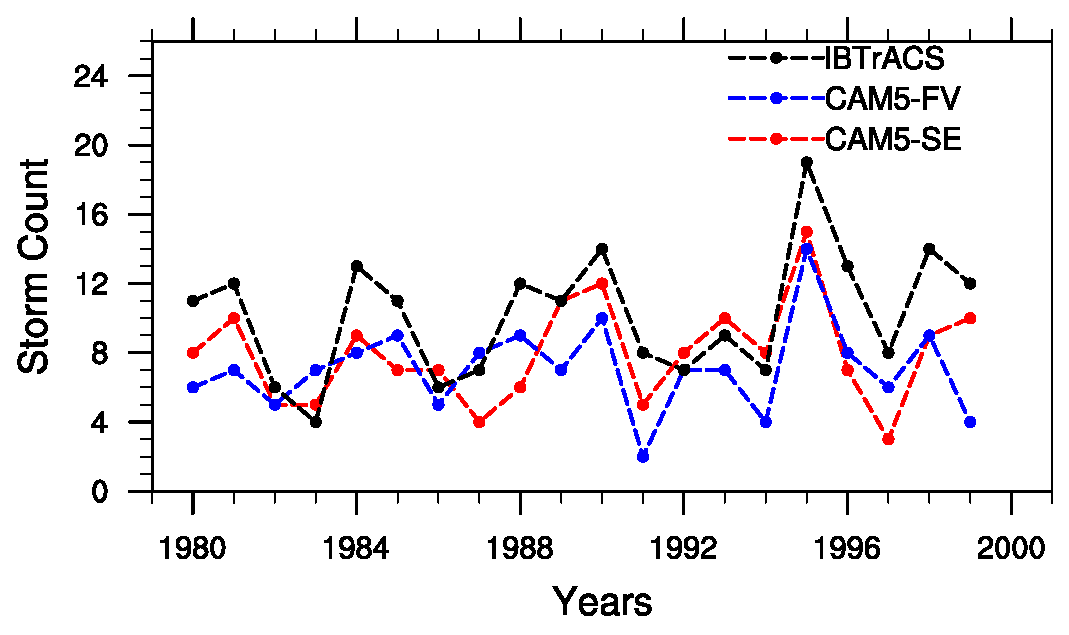
\includegraphics[width=5.in]{NA_interannual.eps}
%\hline
%\end{tabular}
\end{center}
\caption{Annual global tropical cyclone counts simulated from two configurations of the high-resolution CAM5 compared to the observed counts from 1980 to 2000 in the North Atlantic ocean basin.} \label{fig:NATCs}
\end{figure}

\subsubsection{High-throughput event detection with TempestExtremes} \label{sec:TempestExtremes}

The TempestExtremes software package is a new suite of flexible detection and characterization algorithms developed by the Co-PI for processing large climate datasets. This package uses an algorithmic framework known as ``MapReduce'' to first detect candidate events at individual times using specified criteria. Stitching is then used to track pointwise and areal detections in time. The result is a catalog of extreme weather events and associated characteristics whose generation can be automated and parallelized for multiple datasets.

\begin{figure}[ht]
\begin{center}
%\begin{tabular}{|p{4in}|}
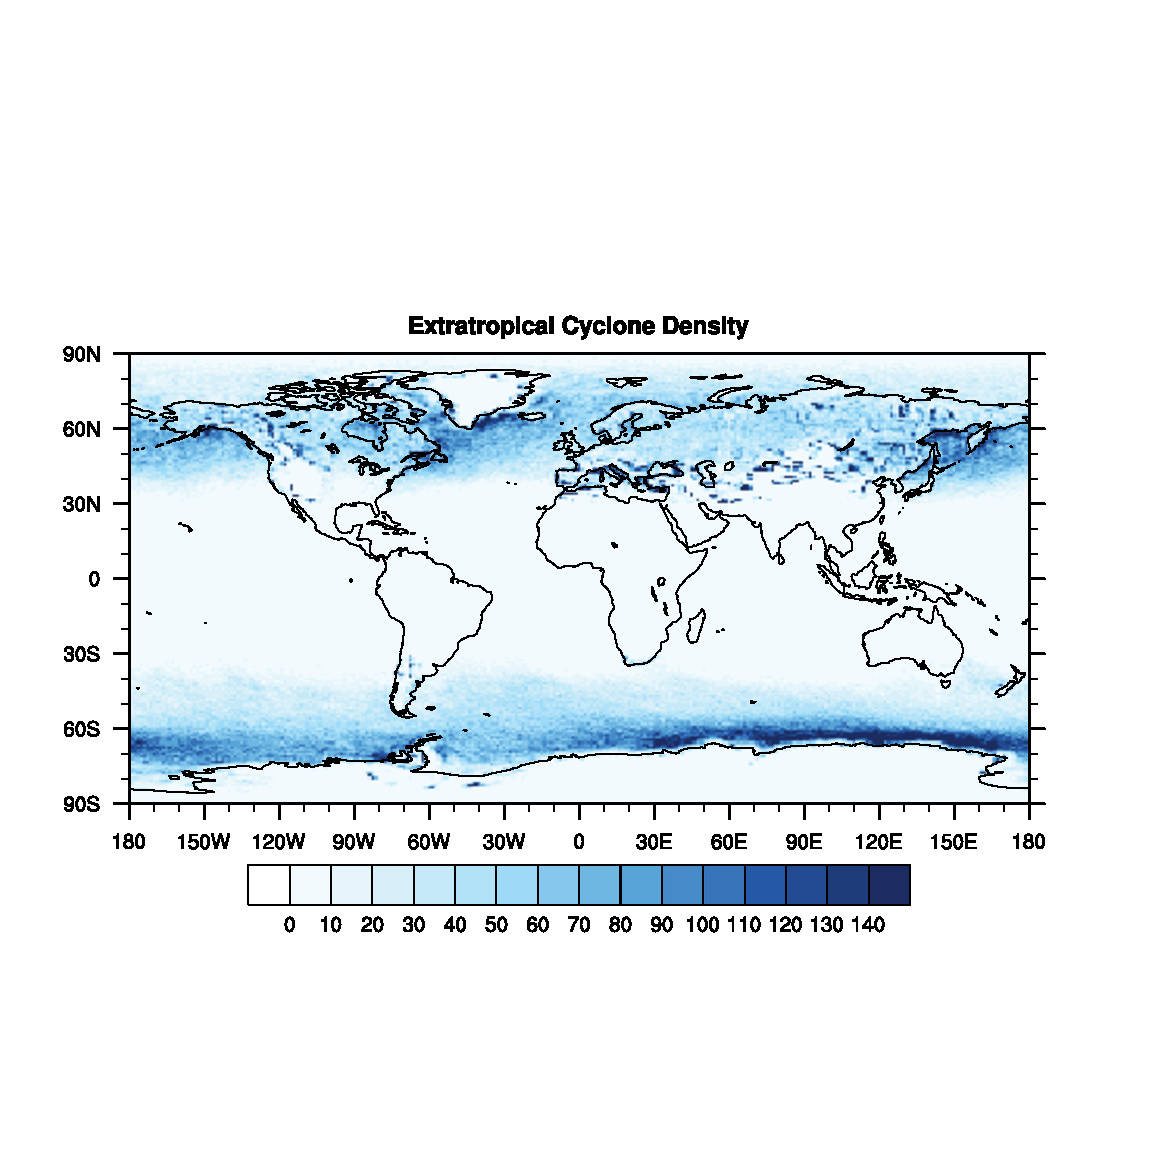
\includegraphics[trim=0.5cm 3.5cm 1cm 4.5cm, clip=true, width=4.5in]{density_plot}
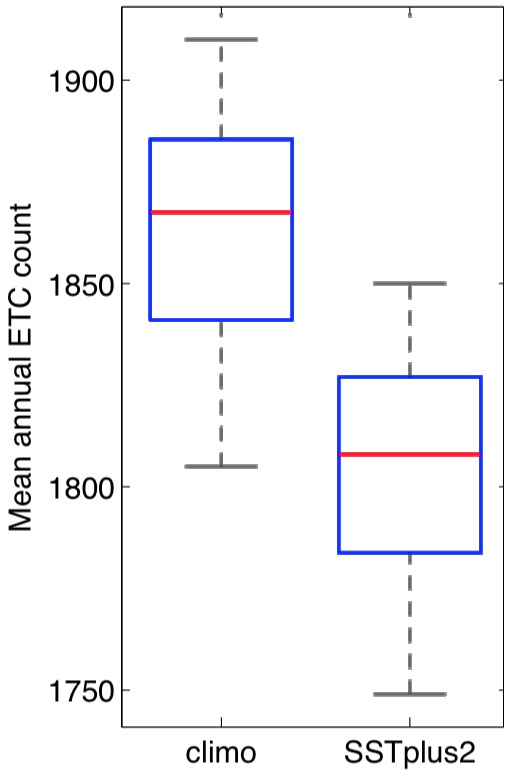
\includegraphics[width=1.5in]{ETCChanges.png}
%\hline
%\end{tabular}
\end{center}
\caption{\textbf{(Left)} Example ETC counts from a 20-year CLIVAR climatological simulation, as obtained by selecting only pressure minima that (a) do not have an upper level warm core, (b) are within 4 degrees of a vorticity maximum, (c) are present over topography of maximum elevation 1500\ m, (d) are persistent for at least 2 days, (e) increase in pressure by  at least 0.1\ hPa over a distance of 1 degree in all directions, and (f) are in the latitude interval [90S, 20S] or [20N, 90N].  \textbf{(Right)} An example of differences between average annual ETC counts from a control simulation (climo) and a simulation with increased sea-surface temperatures (SSTplus2).} \label{fig:DensityPlot}
\end{figure}

In TempestExtremes, detection of both ETCs and TCs is handled by first searching for minima in the sea-level pressure field.  Thresholds can then be specified on the pointwise Laplacian of pressure, maximum or minimum latitude and topographic height at the point of detection.  Additional criteria are also available, including requirement or elimination of candidates based on the presence of a warm core aloft, the presence of a relative vorticity maximum, or the presence of a closed pressure contour.  Once candidate storms have been identified, stitching of candidates to form cyclone tracks is performed.  The stitching algorithm provides options for maximum distance between candidate points, minimum track duration, minimum distance between begin and endpoint, minimum path length, and other user-specified thresholds on quantities such as windspeed or surface pressure.  The stitching algorithm also provides an option for identifying trajectories with detection gaps, for example when candidates are present at times 1,2,3,5,6, and 7.  These criteria amalgamate a wide range of detection and stitching algorithms specified in the literature, and so offer a mechanism for intercomparison of detection criteria.  The use of TempestExtremes for detection and tracking of ETCs has been studied extensively and Figure \ref{fig:DensityPlot} shows the results of ETC densities for two of CAM5 CLIVAR configurations.  Testing of the algorithm for TC tracking is already underway, and shows results consistent with other popular tracking schemes, such as the GFDL tracker. This proposal will apply this detection and stitching technology to the datasets in Section \ref{sec:Datasets} so as to isolate historical and projected trends of North Atlantic cyclone characteristics, and improve statistical confidence in previously reported trends.  Further, this proposal will provided added functionality for detection and tracking of AEWs to TempestExtremes, and so allow tracking of tropical cyclones from their potential origin as AEWs.

\begin{comment}
\subsubsection{Observation and Reanalysis products}\label{sec:Datasets}

{\color{red} We don't really mention this at all...}

Reanalysis products represent climate model hindcasts which are tightly constrained to known observational data.  Development of these products has been a major research focus, particularly over the past decade, with more than half a dozen agencies now maintaining reanalysis datasets.  However, these datasets have the potential to differ significantly depending on the choice of model, specific model parameters, the number of observations and the methodology by which data is assimilated into the model.  Although several major reanalysis products are available, this proposal aims to focus on results from NCEP \citep{kalnay1996ncep}, ERA-40 \citep{uppala2005era}, ERA-Interim \citep{simmons2007era}, MERRA \citep{rienecker2011merra} and C20C \citep{compo2011twentieth}.  The use of multiple datasets is important for identifying and overcoming biases associated with specific atmospheric models that may contaminate the results \citep{jun2008spatial}, and will lead to a set of more robust scientific conclusions. For tropical cyclones, observations from the International Best Track Archive for Climate Stewardship (IBTrACS, \citet{Knapp2010}) for the same time period (1980-2005) will be used. The dataset, endorsed by the World Meteorological Organization, merges tropical cyclone information, including tracks and intensity, from numerous international meteorological centers into a single dataset.
\end{comment}

\subsection{Research Milestones} \label{sec:ResearchMilestones}

The research milestones advanced by this proposal are described in the following sections, along with relevant scientific questions that will be answered over the course of the project.  All tasks will incorporate both validation with present-day climatology and assessments under changing future climate.  The approach described here is a novel assessment of the characteristics of tropical cyclones (and associated AEWs and ETCs) in current and future CAM5 simulations.  The research milestones are separated below into four tasks based on the period of tropical cyclone lifetime, beginning with cyclogenesis, mid-life, extratropical transition and landfall.

\subsubsection{Task 1: African Easterly Waves and Cyclogenesis} 

\begin{figure}[h]
\begin{center}
%\begin{tabular}{|p{4in}|}
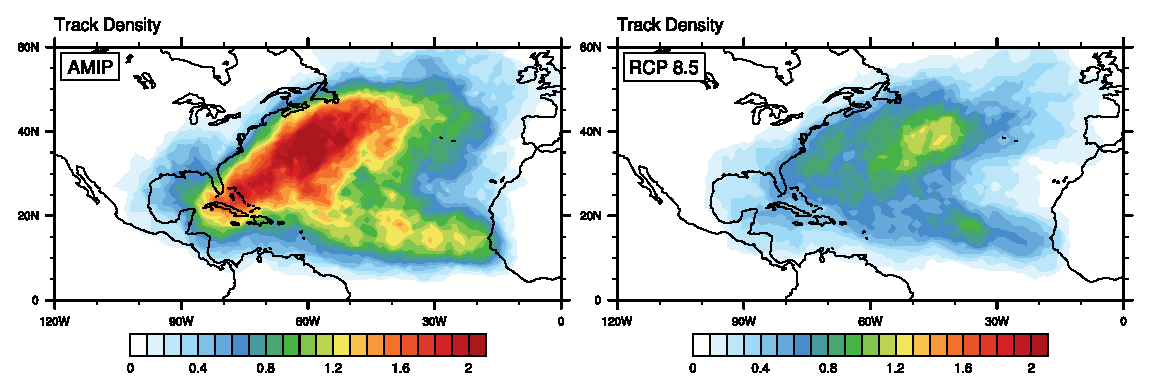
\includegraphics[width=6.in]{NA_track_density.eps}
%\hline
%\end{tabular}
\end{center}
\caption{Preliminary comparison of simulated North Atlantic tropical cyclones track density (average storms per year) for the CAM5-SE AMIP and RCP 8.5 simulations.} \label{fig:NA_density}
\end{figure}

This task investigates the impact of climate change on the behavior of cyclogenesis in the Atlantic basin.  Preliminary work has shown a noticeable decrease in the formation of tropical cyclones in the North Atlantic in CAM5-SE simulations.  Figure \ref{fig:NA_density} shows the track density of TCs for present-day and future simulations using the TC detection algorithm and tracker of \citet{Zhao2009}. The figure indicates a decrease in TCs basin-wide with the largest decrease in the eastern part of the basin off the coast of Africa. The track densities are calculated similar to \citet{Done2013} and defined as the number of TC tracks within a 5 degree radius of a given point per year. This pattern suggests that there is some connection between the future distribution of TCs and AEWs.  Consequently, this task will address the following question:

\textit{Is the location of tropical cyclogenesis in the North Atlantic basin modified under climate change in high-resolution climate model simulations? How does the projected intensification of the African Easterly Jet impact cyclogenesis off the African coast?}

Using the TempestExtremes framework, this proposal aims to determine how discrete AEW events are captured and transition into TCs in both the idealized CLIVAR experiments and ensemble AMIP simulations using the variable resolution model.  Detection and tracking of AEWs has been historically performed using either meridional velocity \citep{Burpee1974, Reed1977} or vorticity \citep{hodges1995feature, thorncroft2001african} at the 850 hPa or 600 hPa level.  We will implement both tracking techniques in TempestExtremes, and will further investigate the use of sea-level pressure minima as an alternative tracking strategy.  The tracking algorithm will be limited to the region $[5^\circ N, 25^\circ N]$ and $[5^\circ W, 35^\circ W]$ in order to prevent spurious detection of non-AEW activity.  In conjunction with the TC detection scheme described in Section \ref{sec:TempestExtremes}, this approach will allow us to identify TC precursors in the form of AEWs and determine what role the strength of AEWs plays in triggering cyclogenesis.  As pointed out by \cite{thorncroft2001african}, AEWs from the southern side of the AEJ play a much greater role in cyclogenesis than AEWs on the poleward side.  Consequently, we will also track the position of the AEJ and determine if our model simulations show any trend in the mean latitudinal position of the jet that may affect the trajectory of AEWs.

This work will focus on characterizing the location and intensity of AEWs, as well as the efficiency of the tropical waves to develop into TCs.  The role of environmental factors, including shear, will also be investigated. It has been hypothesized that changes to the African Easterly Jet as pointed out by \cite{skinner2013contribution}, increased regional temperature gradients and intensification in the strength of convergence and uplift along the Intertropical Front of Africa may lead to an increase in the strength of AEWs.  However, it remains unclear how the frequency of AEWs, and particularly tropical cyclone initiating AEWs will be affected under future climate.

%\cite{hodges1995feature} identifies a technique for tracking AEWs in terms of the vorticity.

%\cite{thorncroft2001african} argue that AEWs on the southern side of the AEJ play a much greater role in tropical cyclogenesis than AEWs on the poleward side.  ``This result suggests that Atlantic tropical cyclone activity may be influenced by the number of AEWs leaving the West African coast, which have significant low-level amplitudes, and not simply by the total number of AEWs.''

%Following \cite{thorncroft2001african}, AEWs will be investigate over the latitudinal range $[5^\circ N, 15^\circ N]$ and $[5^\circ W, 25^\circ W]$.

%: ``We find that increases in regional temperature gradients and the strength of convergence and uplift along the Intertropical Front of Africa lead to increases in the strength of AEWs.''  

%\cite{skinner2012african}: ``Given favorable conditions for cyclogenesis in the eastern Atlantic, AEWs, particularly those associated with convection over West Africa, develop into tropical cyclones.''

%Indeed, nearly all models simulate an increase in the occurrence of intense and extremely intense AEWs along the Sahel?Sahara border (Fig. 5). This includes median changes of +2.0 events per season (and +39\%) for intense AEWs, and +0.8 events per season (and +72\%) for extremely intense AEWs.

\subsubsection{Task 2: Tropical Cyclone Intensity, Size and other Characteristics}

This task addresses potential changes in lifetime characteristics of North Atlantic TCs that may be attributed to climate change. Previous work by \citet{Wehner2015} using the high-resolution CAM5 CLIVAR simulations suggests a global reduction in TC frequency in response to the idealized warming. The results also suggest an increase in intense TCs, an increased average storm duration and a poleward shift in genesis and track densities in the warmer scenarios. However, this CAM5 analysis was not performed at the basin level, specifically the North Atlantic. Understanding how the characteristics of TCs in the North Atlantic will change in the coming century is critical to coastal communities and the U.S. as a whole. Preliminary, CAM5-SE results (see Figure \ref{fig:NA_density}) do suggest that there is a clear decrease in North Atlantic storm count. While numerous studies have investigated the impact of enhanced greenhouse gas forcing on some characteristics of TCs in the North Atlantic \citep[e.g.,][]{Semmler2008,Knutson2008,Zhao2009,Knutson2013,Done2013,Diro2014}, such studies have typical been performed with regional models and/or at coarser horizontal resolutions than the 25 km grid spacings proposed here.  Therefore, this task will address the following question:

\emph{How are the lifetime characteristics of tropical cyclones, including wind intensity, size, precipitation, and spatial density of storms affected under future climate change in high-resolution climate model simulations?}

Previous studies of TCs at high-resolution in climate models are typically limited to one realization (i.e. one ensemble member). As mentioned in Section \ref{sec:CAM-data}, only recently have ensemble simulations been completed in the CAM5-FV AMIP configuration for the period of 1995 to 2005 in collaboration with Michael Wehner at LBNL. In addition, with the proposed CAM5-SE AMIP and RCP 8.5 ensemble simulations offer a unique opportunity to study changes North Atlantic tropical cyclone climatology. Utilizing the enhanced TempestExtreme framework the characteristics of TCs will be explored in the various CAM5-SE and CAM5-FV AMIP configurations. Making use of this large high-resolution ensemble will allow for a robust analysis of the impact of a warming climate on North Atlantic TC intensity, track duration, precipitation and track distribution. 

Additionally, the proposed work will perform the first analysis of TC size using CAM5 simulations. In particular, the size algorithm described in \cite{Chavas2014} will be implemented to study TC size in the present day AMIP and CLIVAR simulations, as well as changes in size in the future warming scenarios. Recent work by \citet{Kim2014}, using a coupled global model at 50 km horizontal resolution, suggests that the average TC size will increase by 3\% under a doubling of carbon dioxide. While a study by \citet{Lin2015} suggests that TC size, as defined by rainfall area, is not expected to change significantly in a warmer climate. Understanding how the size of TCs will be altered in the future is crucial, as TC size has implications for storm damage and the area which experience strong winds and influences the extent of storm surge \citep{Powell2007}. Hurricane Sandy of 2012 is a perfect example of the magnitude of damage larger sized storms can inflict. The proposed analysis is novel for CAM5 and at these resolutions.
 
\subsubsection{Task 3: Characterization of the Extratropical Transition}

The extratropical transition of tropical cyclones is an important meteorological phenomenon whereby warm-core TCs transition into cold-core ETCs when they are sufficiently far from the tropics.  The extratropical transition has been studied in the meteorological literature, and is fairly well understood \citep{hart2001climatology}.  However, the extratropical transition has not been thoroughly investigated in the context of climate change.  Although studies on the effects of future climate have largely concluded that tropical cyclones will generally be fewer in number but more intense \citep{Knutson2010}, past studies of ETCs have stated that although ETCs will be fewer in number, only precipitation intensity is expected to increase \citep{bengtsson2009will}.  Consequently, it is worthwhile to examine the influence of the changing climate on ETCs which occur due to extratropical transition of tropical cyclones in the North Atlantic using the infrastructure developed as part of proposed question:

\emph{Is there a change in the character, including location and frequency, of tropical cyclones undergoing an extratropical transition?}

TempestExtremes offers the unique ability to track tropical cyclones and extratropical cyclones under one framework, and as a result offers the ability to capture cyclones that undergo extratropical transition in the North Atlantic basin.  TempestExtremes has been shown to be reliable in detecting and tracking ETCs (see Fig. \ref{fig:DensityPlot}), and can be employed to isolate only ETCs that originate from the transition of tropical cyclones. The process of extratropical transition has not previously been studied using CAM5, as high-resolution simulations are required to capture the precursor tropical cyclones. Therefore, the proposed work will be the first high-resolution modeling study on the number of tropical cyclones that undergo extratropical transition, as well as the intensity, location and distribution of such cyclones.  

In order to perform this analysis, the proposed ensemble CAM5 CLIVAR and AMIP simulations will be crucial.  Observations indicate that on average 46$\%$ of tropical cyclones undergo extratropical transition in the North Atlantic \citep{hart2001climatology}. Given the relatively low annual number of North Atlantic tropical cyclones in observations and model results (and therefore the even lower frequency of cyclones undergoing extratropical transition) the large ensembles will be needed to obtain adequate statistics.

As mentioned earlier, previous work has largely focused on potential changes to North Atlantic TCs and ETCs in isolation.  Consequently, little is known to how the process of extratropical transition will be altered. Recent events, including Hurricane Sandy, have brought a renewed interest to the extratropical transition and the devastating impacts that transitioning cyclones can have on the East Coast of the United States \citep{Blake2013}. As stated, previous and preliminary work with CAM5 has indicated that the number of TCs in the North Atlantic will decrease under future warming scenarios. This may suggest a decrease in the number of TCs that undergo extratropical transition.  However, \citet{Wehner2015} suggests that due to warmer sea surface temperature the duration of TCs has increased globally in the  CLIVAR simulations.  This observation indicates that the ability of TCs to reach regions where extratropical transition occurs may increase.

The proposed work will shed new light on this subject area by making use of the CAM5 ensemble simulations for both present day and future climate forcing. Combined with the previous task for TCs, the proposed work will qualify future trends in tropical cyclone intensity, tracks and duration and the implications of such trends for extratropical transition in the North Atlantic.

\subsubsection{Task 4: Characterization of Landfalling Cyclones}

Landfalling storms cause the most direct impact on the United States and throughout North America.  They are the costliest of natural disasters in the United States \citep{Pielke1998}, with a disproportionate expense coming from individual storms that are particularly intense, large in size or that impact vulnerable regions. Recent examples of destructive storms include Hurricane Katrina (2005) and Hurricane Sandy (2012). As mentioned in Task 2, storm size has serious ramifications for damage potential to coastal communities, in addition to the well-known impact of cyclone intensity.  The overland precipitation of landfalling tropical cyclones also poses a threat to the continental United States through major flooding events \citep{Villarini2014tcflooding}. Recent work by \citet{Scoccimarro2014} and \cite{Villarini2014} using multi-model ensembles from CLIVAR HWG (the latter including the CAM5 CLIVAR runs) suggest that rainfall associated with TCs will increase in a warming climate. The proposed work will address the following question using the CAM5 ensemble simulations:

\emph{How are cyclone trajectories, probability of landfall, location of landfall and total overland precipitation affected under future climate change?}

By using the unified TempestExtreme framework for cyclones in the North Atlantic, this project will enable a detailed investigation of landfalling cyclones.  Utilizing the present and future CAM5 ensemble simulations the analysis will include diagnosing changes in the intensity, size and precipitation of landfalling cyclones in the future climate scenario. Recent work using a beta and advection model by \citet{Colbert2013} suggests that human-induced climate change will alter tropical cyclone tracks in the North Atlantic, leading to a decrease in straight-moving westward storms and and increase in recurving storms over the ocean due to changes in the large-scale dynamics.  This work indicates that there is no change in the overall frequency of recurving landfalling storms, but suggests there may be more localized shifts in the landfall distributions. Our analysis will investigate the frequency and distribution and characteristics of landfalling TCs and ETCs under future climate change. The proposed project will investigate whether there are changes in the frequency of transitioning TCs that can also have significant impacts on coastal communities.  By further incorporating storms that are undergoing extratropical transition, the research will offer new insights into the full range of potential climate impacts of cyclones in North Atlantic coastal communities.

\subsection{Timeline} \label{sec:Timeline}

The graduate student researchers will tackle the problem of TC lifecycle from each end:  One student, under the direction of Co-PI Paul Ullrich, will implement and evaluate tracking capability of AEWs and study the effect of changing AEWs on tropical cyclogenesis and into early lifetime.  One student, under the direction of PI Kevin Reed, will focus on the termination of cyclones either through extratropical transition or via landfall.  Both students will work on addressing the characteristics of TCs.  Substantial collaboration is expected between investigators, and will be facilitated via online meetings every two weeks and in-person meetings at conferences.  The approximate timeline is as follows:

\begin{tabularx}{\textwidth}{cX}
\hline
\\
\textbf{Year 1} & $\cdot$ Implement AEW tracking capability in TempestExtremes. \\
& $\cdot$ Further test TC tracking TempestExtremes on CAM5 CLIVAR simulations. \\
& $\cdot$ Setup and start CAM5-SE present-day and RCP8.5 variable resolution ensemble runs. \\
& $\cdot$ Implement TC to ETC tracking on existing CAM5 runs, as well as TC size algorithm.\\ 
\\
\hline
\\
\textbf{Year 2} & $\cdot$ Complete CAM5-SE present-day and RCP8.5 variable resolution ensemble runs.  \\
& $\cdot$ Test and apply AEW TempestExtremes tracking to CAM5 model data. \\
& $\cdot$ Implement TC to ETC tracking on CAM5-SE ensemble runs.\\
& $\cdot$ Complete analysis of genesis and AEW characteristics (Task 1) with journal article. \\
& $\cdot$ Complete investigation of TC characteristics (Task 2) with journal article. \\
\\
\hline
\\
\textbf{Year 3} & $\cdot$ Complete analysis of extratropical transition characteristics (Task 3) with article. \\ 
& $\cdot$ Complete investigation of cyclone landfalling change (Task 4) with journal article. \\
& $\cdot$ Write overview article introducing lifecycle detection framework for large datasets. \\
\\
\hline
\end{tabularx}

We anticipate that multiple major peer-reviewed publications will arise from this work, addressing the studies of detection, attribution and prediction. Further, this work will be presented at major scientific meetings, including the annual meetings for the American Meteorological Society, the European Geophysical Union and the American Geophysical Union.

\subsection{Online access to climate data and results}\label{sec:data access}

Dissemination of climate data and scientific results is an important issue for increasing public understanding of climate change.  To this end, we anticipate releasing all variable resolution model runs completed by this project via the Earth System Grid (\texttt{https://www.earthsystemgrid.org/}).  All software produced in conjunction with the project (including the AEW, TC and ETC detection capability in TempestExtremes) will be released under the open source Lesser GNU Public License (LGPL), so as to be available for use by other investigators.  The software will be available for public download via GitHub.  We further plan to release a summary of all results from this work for public consumption.

\subsection{Strengths of the team}\label{sec:strengths}

The PI, Co-PI and their collaborating team are uniquely positioned to conduct multi-model ensemble intercomparisons, including variable-resolution configurations, of climate model output using a suite of cutting-edge atmospheric models and post-processing tools.

PI Kevin Reed brings considerable experience in high-resolution climate modeling.  His past research has focused on understanding the ability of the Community Atmosphere Model (CAM) to simulate tropical cyclones at present-day and next-generation horizontal resolution \citep{Reed2011a,Reed2011c,Reed2012b}.  This includes the study of how tropical cyclones and precipitation extremes change with climate change using decadal climate simulations at approximately 25-km horizontal resolution \citep{Wehner2014,Villarini2014,Wehner2015,Reed2015b}. Prof Reed also has developed techniques to utilize reduced complexity testbeds for understanding cloud, circulation and precipitation sensitivities in General Circulation Models (GCMs) \citep{Reed2012a,Reed2015a}. These simplified techniques have shown to be useful to rationalize robust behaviors of the Earth system and are vital to continued model development and intercomparison. Through his work, Prof. Reed has developed international collaborations in model development and high-resolution modeling.

This project will further benefit from Co-PI Ullrich's experience with atmospheric model development  (\cite{ullrich2010high, PHLPAURDN2011SPRINGER, ullrich2012operator, ullrich2012mcore, ullrich2014fluxform, guba2014viscosity, ullrich2014understanding, ullrich2014global}), numerical analysis (\cite{ullrich2011analysis, ullrich2012considerations}) and model evaluation (\cite{DCMIP2012TESTCASES, ullrich2014proposed, kent2013dynamical, ullrich2014baroclinic}).  PI Ullrich has been heavily involved with work on variable-resolution modeling \citep{zarzycki2014aquaplanet} and adaptive mesh refinement  \citep{collins2013nonhydrostatic, mccorquodale2014adaptive}. Many relevant tools have been developed by the Co-PI, including the SQuadGen grid generation tool (described in \cite{guba2014viscosity}), the TempestRemap post-processing toolkit \citep{ullrich2015remapping} and the TempestExtremes toolkit for extreme weather detection and characterization \citep{ullrich2015extremes}. He is heavily involved in national collaborations on climate projects, and is an organizer on a number of sessions and workshops which are related to atmospheric modeling. In addition, he is closely affiliated with ongoing climate research efforts at Lawrence Berkeley National Laboratory (LBNL) and the National Center for Atmospheric Research (NCAR).

In addition to the funded investigators, the project will also incorporate close collaborations with expert scientists involved in the development, simulation and analysis of high-resolution CAM5.  In particular, Dr. Michael Wehner at the Department of Energy Lawrence Berkeley National Laboratory will provide the CAM5-FV AMIP and CLIVAR model data and aid in the analysis of TCs for the proposed work.  Dr. Wehner has considerable expertise in running 25 km simulations with numerous versions of CAM. Furthermore, Dr. Julio Bacmeister at NCAR is heavily involved with the development of the high-resolution versions of CAM5-SE and will provide access to the CAM5-SE AMIP simulations that were performed under his direction.  In addition, Dr. Bacmeister will aid in the set up of the proposed CAM5-SE ensemble simulations. These collaborations, as well as new ones that will be formed over the course of the project, will help ensure the success of the proposed research. 

{\setbox0\vbox{\bibliography{NSFCyclones-Bibliography}}}
\bibliographystyle{wileyqj}

\end{document}
